\chapter{ジャンル境界の可視化}
\label{chapter4}章で構築した学習済みGeneratorにおいて,入力される128次元のランダムノイズベクトルの値を固定し,従属関係にある10次元のベクトルの中から特定の二つのベクトル次元の値を変化させていく.このときに生成したスペクトログラムをジャンル分類することにより,二次元特徴マップ空間として可視化する.またその時のスペクトログラムを可視化する.

\section{二次元特徴マップ可視化}
従属関係にある入力ベクトルとジャンル出力との関係を二次元特徴マップ空間により可視化する.初めに初期値として$-$1~1の一様分布に従うランダムノイズを128次元生成する.(\figref{fig:randomnoise})次に従属関係にある10次元のベクトル$c$から2次元だけを取り出しその値を変化させいく.(\figref{fig:variablenoise})すると,値の変換に応じて生成するスペクトログラムとジャンル分類結果が変化するため,その時の2次元ベクトルの値とジャンル分類結果を特徴マップにプロットしていく.(\figref{fig:featmap})

\begin{figure}
	\begin{center}
		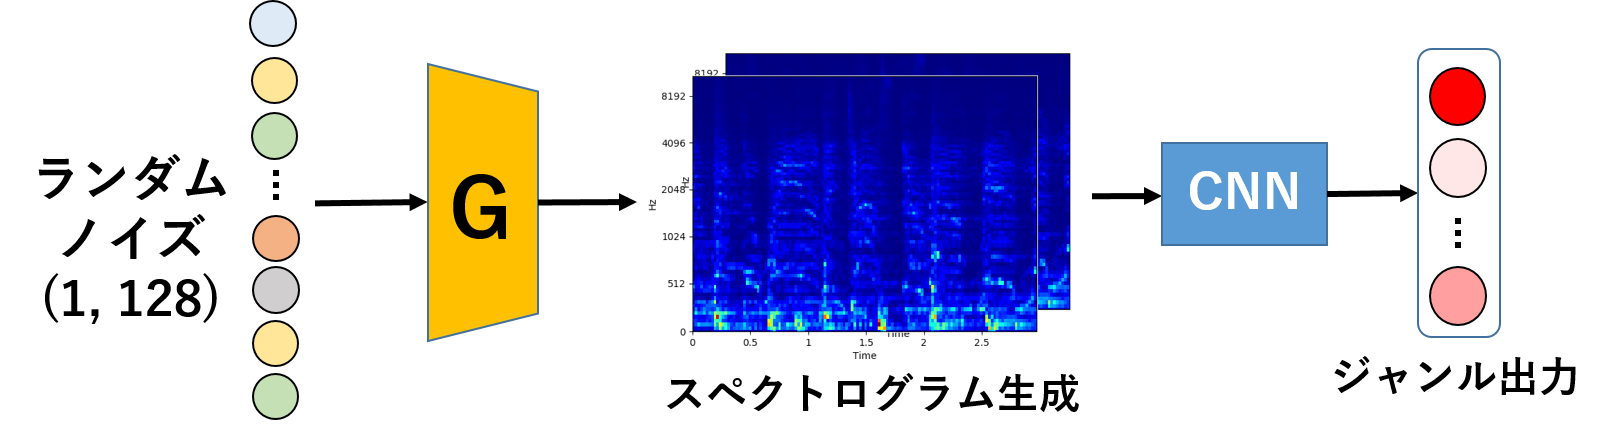
\includegraphics[scale=0.5]{./images_ch-visualize/randomnoise.png}
		\caption{初期値ランダムノイズ生成}
		\label{fig:randomnoise}
	\end{center}
\end{figure}
\begin{figure}
	\begin{center}
		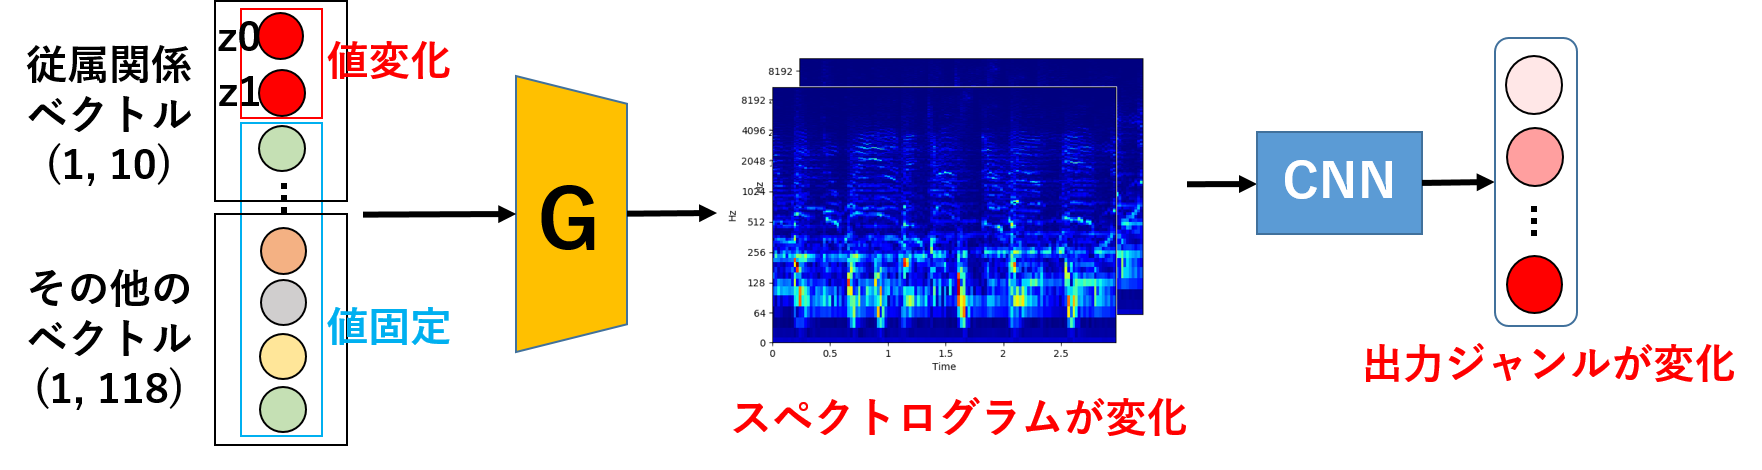
\includegraphics[scale=0.5]{./images_ch-visualize/variablenoise.png}
		\caption{従属関係のベクトル値を変化}
		\label{fig:variablenoise}
	\end{center}
\end{figure}
\begin{figure}
	\begin{center}
		\includegraphics[scale=0.7]{./images_ch-visualize/map1.png}
		\caption{二次元特徴マップ空間}
		\label{fig:featmap}
	\end{center}
\end{figure}


\section{ジャンル出力確率と生成スペクトログラムの変化}

\subsection{ジャンル出力確率の変化}
\figref{fig:featmap-trans}のように,二次元特徴マップ空間において,矢印の方向でジャンル境界を跨ぐように座標をずらしていき,そのときのジャンル出力確率の変化をグラフにしたものを\figref{fig:trans-graph}に示す.
\begin{figure}
	\begin{center}
		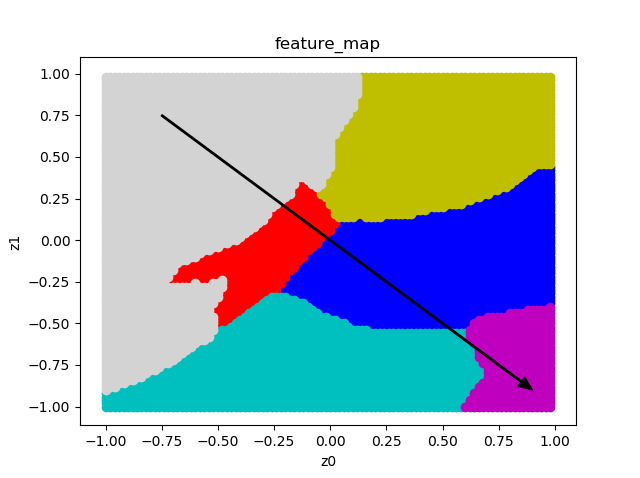
\includegraphics[scale=0.5]{./images_ch-visualize/map_trans.png}
		\caption{ジャンルデータの変化}
		\label{fig:featmap-trans}
	\end{center}
\end{figure}
\begin{figure}
	\begin{center}
		\includegraphics[scale=0.7]{./images_ch-visualize/prob_feat.png}
		\caption{ジャンル毎の確率変化}
		\label{fig:trans-graph}
	\end{center}
\end{figure}

ジャンル同士の出力確率が連続変化していることから,生成されるスペクトログラムはジャンルの特徴となるものが連続変化をしていると言える.また,ジャンルの一方が上がり一方が下がるということから,一つのジャンルのみに依存する特長があるということがわかり,交差する点がジャンル境界となるため,その時のスペクトログラムがジャンル中間データとなりうると考えられる.